\section{Sensoren}

\subsection{Schalter}
    \begin{itemize}
        \item Vorteile 
            \begin{itemize}
                \item Einfach und Kostengünstig
                \item Hohe Lebensdauer
                \item Hohe Spannungen und Ströme schaltbar
            \end{itemize}
        \item Nachteile 
            \begin{itemize}
                \item Prellen / Kleben
                \item Langsam
            \end{itemize}
    \end{itemize}

    \textbf{Entprellen durch:} 
    
    \begin{minipage}{0.48\columnwidth}
        Tiefpass + Schmitt-Trigger:
        \begin{figure}[H]
            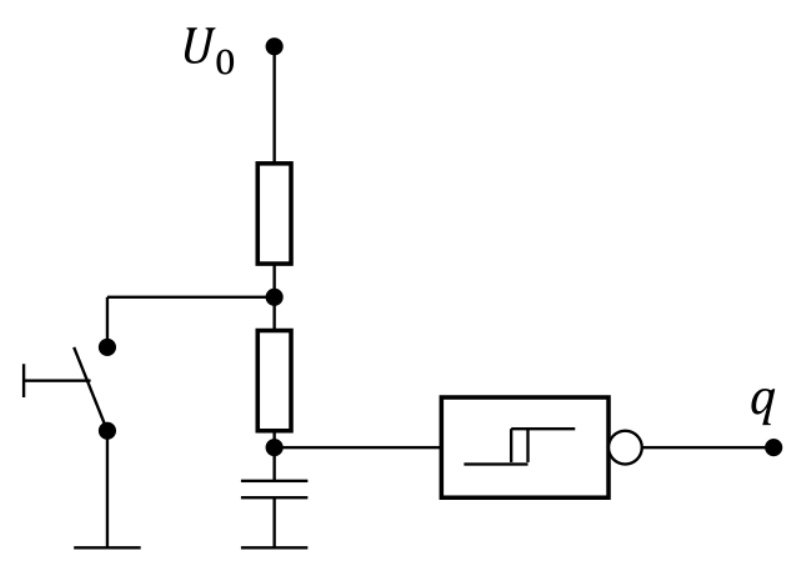
\includegraphics[width=0.98\textwidth]{Figures/sensoren/schalter_schmitt.png}
        \end{figure}
        wobei: \(RC > Prelldauer\)     
    \end{minipage}
    \hfill
    \begin{minipage}{0.48\columnwidth}
        Verriegelungsschaltung:
        \begin{figure}[H]
            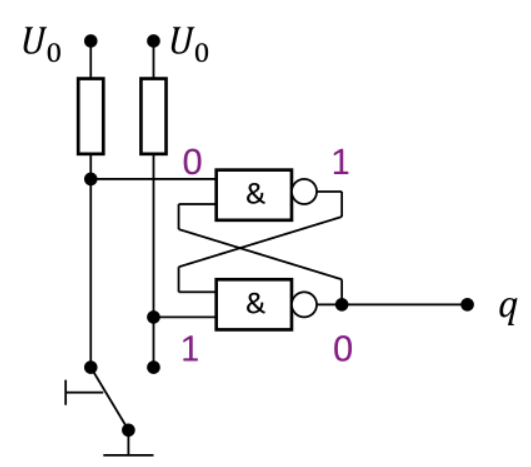
\includegraphics[width=0.98\textwidth]{Figures/sensoren/schalter_verriegelung.png}
        \end{figure}    
    \end{minipage}

\subsubsection{Lichtschranke}
    \begin{itemize}
        \item Vorteile 
            \begin{itemize}
                \item Berührungslos, keine Rückwirkung auf Messobjekt
                \item Sehr hohe Lebensdauer, verschleißfrei
                \item relativ Kostengünstig
                \item Hohe Schaltgeschwindigkeit
            \end{itemize}
        \item Nachteile 
            \begin{itemize}
                \item Lichtweg darf nicht gestört werden (Absorption, Streuung)
                \item Störlichtquellen (Sonne, andere Lampen)
            \end{itemize}
    \end{itemize}

\subsection{Winkel- und Längenmessung}
    \subsubsection{Potentiometer}
        \begin{figure}[H]
            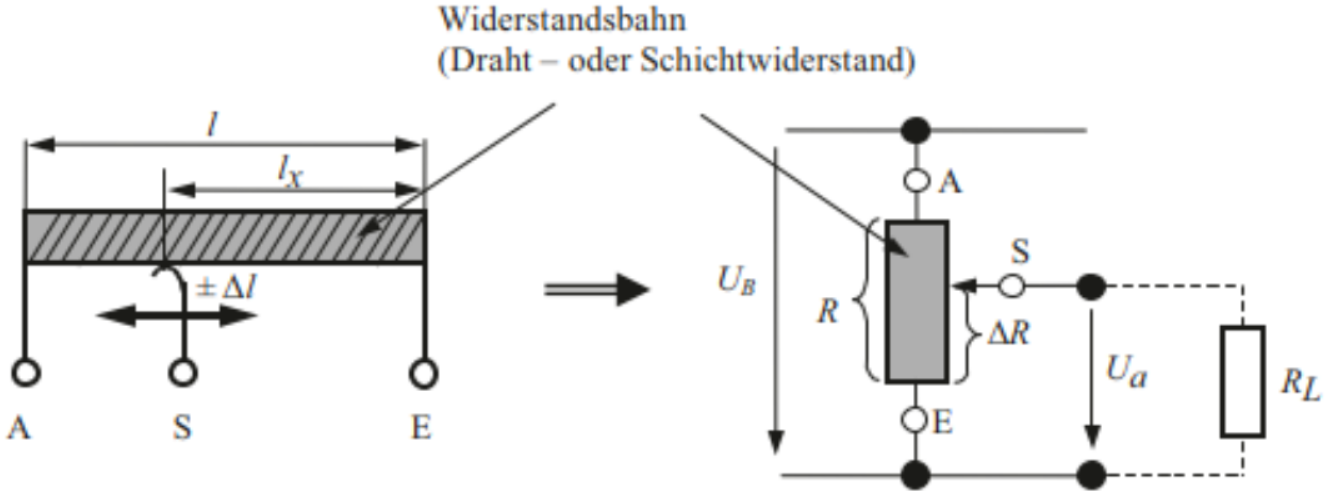
\includegraphics[width=0.9\columnwidth]{Figures/sensoren/poti_schiebe.png}
        \end{figure}
        \begin{align*}
            U_a &= U_B \cdot \frac{\Delta R}{R} \\
            \Aboxed{
                U_a &= U_B \cdot \frac{l_x}{l} = U_B \frac{\alpha}{\alpha_0}
            }
        \end{align*}
        \textbf{Bei Belastung des Spannungsteilers wird der Messwert verfälscht}

    \subsubsection{Inkrementalgeber}
        \begin{figure}[H]
            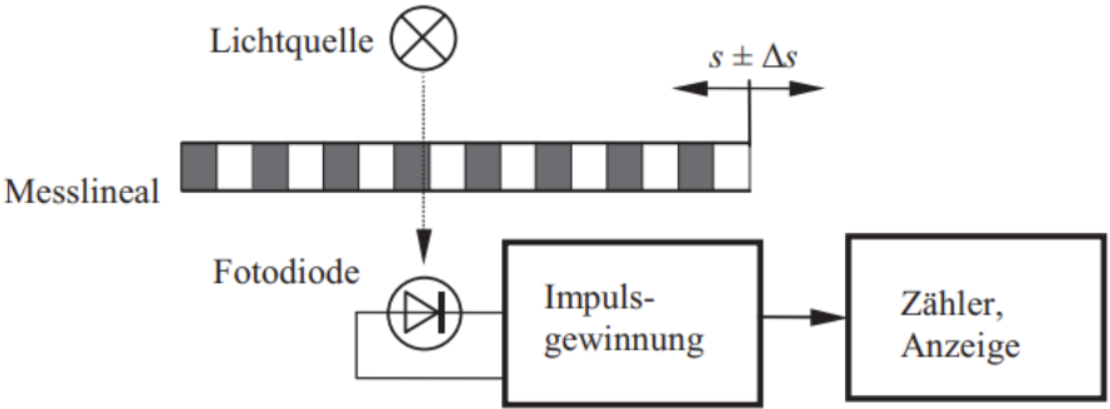
\includegraphics[width=0.9\columnwidth]{Figures/sensoren/inkrementalgeber.png}
        \end{figure}
        \begin{itemize}
            \item Messprinzip 
                \begin{itemize}
                    \item Zählung der hell/dunkel Phasen der Fotodiode
                    \item Die Längenauflösung beträgt \(\Delta s\) (1 Periode des Messlineals)
                \end{itemize}
            \item Vorteile 
                \begin{itemize}
                    \item relativ einfach
                    \item Sensor berührungslos
                \end{itemize}
            \item Nachteile 
                \begin{itemize}
                    \item Hier keine Richtungserkennung möglich
                    \item Keine absolute Positionsmessung
                    \item Für abs. Position muss bekannte Referenzposition angefahren werden.
                    \item Synchronisation der Bitwechsel bei 2 Messlinealen \textrightarrow Gray-Code
                    {\small
                        Generierung Gray-Code\\
                        X1: Dualzahl im Binärcode\\
                        X2: X1 >> 1 (Rechtsshift um 1)\\
                        Gray-Code X3: X1 xor X2
                    }
                \end{itemize}
        \end{itemize}

        \textbf{Verbesserung durch 2 Messlineale, welche } \(\frac{\Delta s}{4}\) \textbf{verschoben sind.}
        {\footnotesize s. Sensoren S. 17}

        Drehzahlmessung:
        \begin{itemize}
            \item Zählung der Impulse \(N\) in fester Zeit \(T\): \\
                \(\omega = \frac{\Delta \varphi \cdot N}{T}\) \\ 
                Auflösung: \(\Delta \omega = \frac{\Delta \varphi}{T}\)
            \item Messung der Zeitdifferenz zwischen zwei folgenden Pulsen: \\
                \(\omega = \frac{\Delta \varphi}{T}\) \\
                Auflösung: \(\Delta \omega = \frac{\Delta \varphi}{T^2} \cdot \Delta T\)
        \end{itemize}
    
\subsection{Temperaturmessung}
    \subsubsection{Widerstände}
        \begin{itemize}
            \item Pt100: Platin-Widerstandsthermometer mit 100 \(\Omega\) bei 0 °C
            \item Pt1000: Platin-Widerstandsthermometer mit 1000 \(\Omega\) bei 0 °C (Vorteil: Geringerer Fehler durch Leitungswiderstand)
        \end{itemize}
        \begin{align*}
            R(\vartheta) &= R_0 \cdot (1 + \alpha \cdot (\vartheta - \vartheta_0) + \beta (\vartheta - \vartheta_0)^2 + \ldots) \\
            R(\vartheta) &\approx R_0 \cdot (1 + \bar{\alpha} \cdot (\vartheta - \vartheta_0)) \text{ mit } \bar{\alpha} = \frac{R(\vartheta_1) - R(\vartheta_0)}{R(\vartheta_0) \cdot (\vartheta_1 - \vartheta_0)}\\
            &\text{Platin: } \bar{\alpha} \approx 3850 \cdot 10^{-6} \frac{1}{^\circ C}
        \end{align*}
        Auswertung durch Widerstandsmessung: 
        \begin{itemize}
            \item Zweileiter-Messung: \(R_{gemessen} = R_{Pt} + 2 \cdot R_{Leitung}\)
            \item Vierleiter-Messung: \(R_{gemessen} = R_{Pt}\)
        \end{itemize}
        Ansprechzeit: \(t_{0,5}\) bzw. \(t_{0,9}\) Zeit, nach der 50\% bzw. 90\% des Endwerts erreicht sind. (Sprunganregung)\\
        Selbsterwärmung mit Selbsterwärmungskoeffizient \(S\): \(\Delta T = S \cdot P\)
    \subsubsection{Thermodiffusion/Seebeck}
        \begin{itemize}
            \item Benötigen Vergleichstemperatur
            \item Einsatz bei sehr hohen Temperaturen
            \item Ungenauer als Pt100, aber schnelleres Ansprechverhalten
        \end{itemize}
        \begin{figure}[H]
            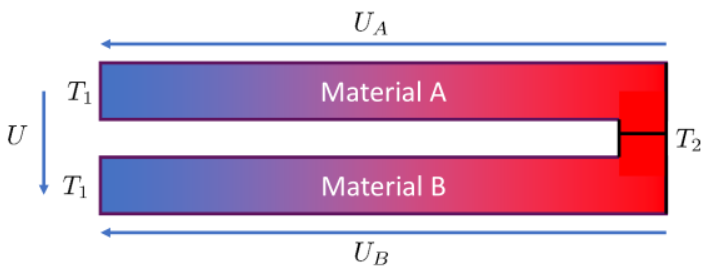
\includegraphics[width=0.9\columnwidth]{Figures/sensoren/thermodiffusion.png}
        \end{figure}
        \begin{align*}
            U \approx (S_B - S_A) \cdot (T_2 - T_1)
        \end{align*}
    \subsubsection{NTC}
        \begin{align*}
            R(\vartheta) = R_0 \cdot e^{B \cdot (\frac{1}{T} - \frac{1}{T_0})} \text{Achtung in Kelvin}
        \end{align*}

\subsection{Kraftmessung}
    \subsubsection{DMS}
        \begin{align*}
            \frac{\Delta R}{R} = \left( \frac{\Delta \rho}{\rho \varepsilon} + 2 \mu + 1 \right) \cdot \varepsilon = k \cdot \varepsilon
        \end{align*}
        \begin{itemize}
            \item Halbleiter-DMS:
                \begin{itemize}
                    \item Sehr hoher \(k\)-Faktor, für hohe Empfindlichkeit
                    \item Stärkere und nichtlineare Temperaturabhängigkeit
                    \item Nichtlinear bei großen Dehnungen
                \end{itemize}
            \item Metall-DMS:
                \begin{itemize}
                    \item Geringerer \(k\)-Faktor (\(\approx 2\))
                    \item lineare Temperaturabhängigkeit
                    \item Linear bei großen Dehnungen
                \end{itemize}
        \end{itemize}
        Messwertverarbeitung:
        \begin{itemize}
            \item Viertelbrücke: \\
                \(U_{AB} \approx \frac{\Delta R}{4R} \cdot U_0 = \frac{U_0}{4} \cdot k \cdot \varepsilon\)
            \item Halbbrücke (unbelasteter Balken): \\
                \(U_{AB} \approx \frac{\Delta R}{4R} \cdot U_0 = \frac{U_0}{4} \cdot k \cdot \varepsilon\) \\
                Vorteil: Temperaturkompensation, da beide DMS die gleiche Temperatur haben
            \item Halbbrücke (selber Balken): \\
                \(U_{AB} \approx \frac{\Delta R}{2R} \cdot U_0 = \frac{U_0}{2} \cdot k \cdot \varepsilon\) \\
                Vorteil: Höhere Empfindlichkeit, Temperaturkompensation (DMS an unterschiedlichen Seiten des Balkens)
            \item Vollbrücke: \\
                \(U_{AB} \approx \frac{\Delta R}{R} \cdot U_0 = U_0 \cdot k \cdot \varepsilon\)
        \end{itemize}

    \subsubsection{Piezoeffekt}
        Ladung direkt proportional zur auf den Sensor wirkenden Kraft:
        \begin{align*}
            Q = k_p \cdot F
        \end{align*}
        \begin{figure}[H]
            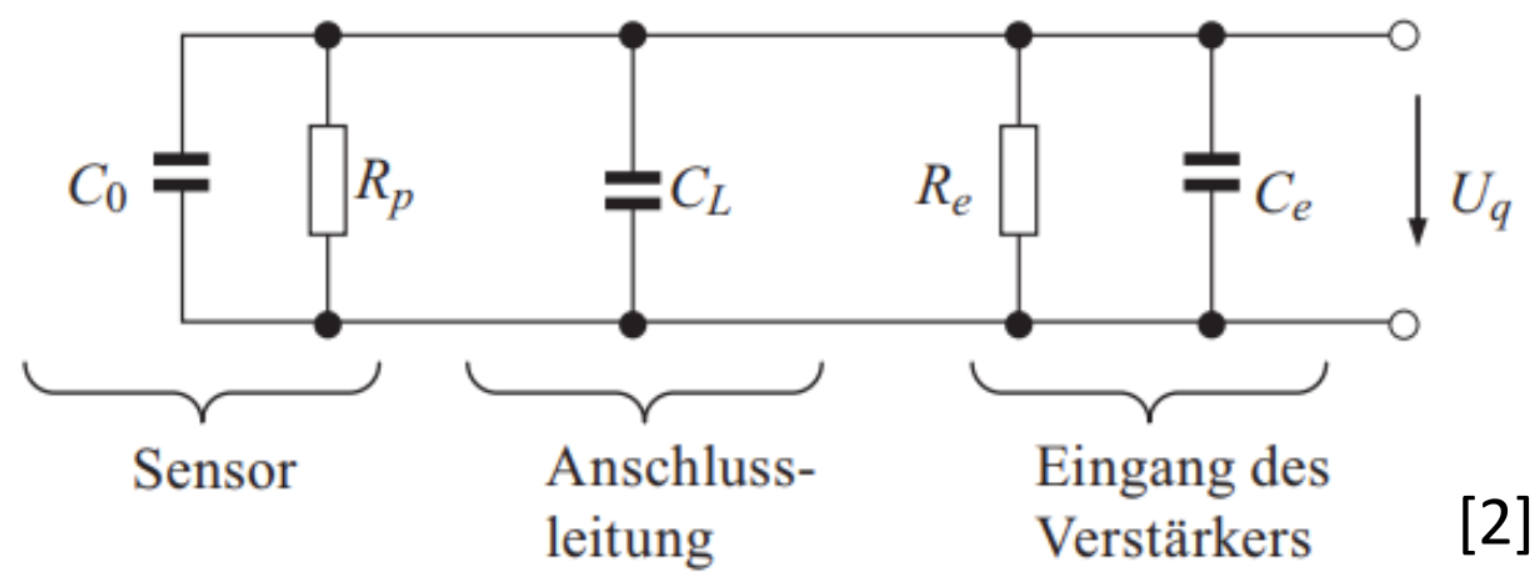
\includegraphics[width=0.9\columnwidth]{Figures/sensoren/piezo_basic.png}
        \end{figure}
        \begin{align*}
            U_q = \frac{Q}{C_{ges}} = \frac{k_p \cdot F}{C_0 + C_L + C_e}
        \end{align*}
        Probleme:
        \begin{itemize}
            \item Messaufbau verändert Empfindlichkeit
            \item Widerstände müssen sehr hoch sein, um Ladung nicht zu entladen (Wertänderung über Zeit, da \(\tau = R_{ges} \cdot C_{ges}\))
        \end{itemize}
        \textrightarrow Messung von veränderlichen Kräften

        \textbf{Ladungsverstärker}
        \begin{figure}[H]
            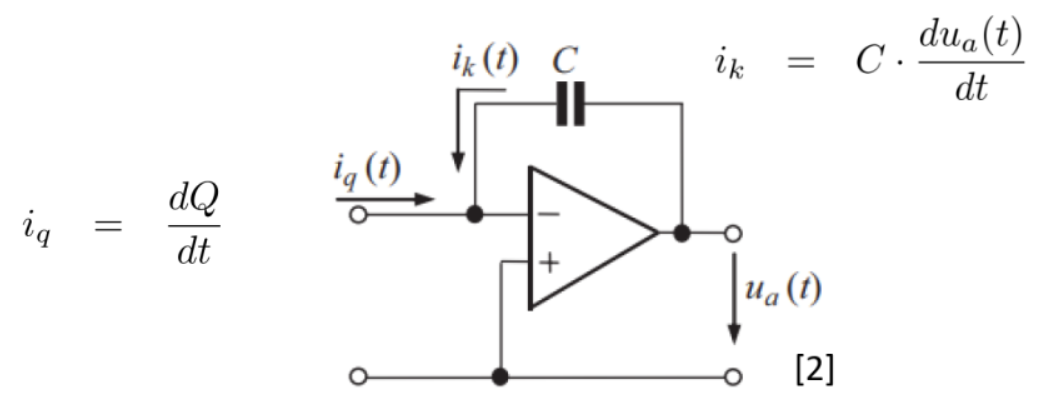
\includegraphics[width=0.9\columnwidth]{Figures/sensoren/piezo_ladungsverst.png}
        \end{figure}
        \begin{align*}
            u_a(t) = - \frac{Q}{C} = - \frac{k_p \cdot F(t)}{C}
        \end{align*}
        \begin{itemize}
            \item Ausgangsspannung unabhängig von parasitären Kapazitäten
            \item Messbereichsanpassung durch Wahl von \(C\)
            \item Entladen von C vor Messung notwendig
        \end{itemize}

\subsection{Druckmessung}
    \begin{align*}
        h &= \frac{T_0}{k_T} \cdot \left[ 1 - \left( \frac{p}{p_0} \right)^{-\frac{k_T R_s}{g}} \right] + h_0 \\
          & \approx 44.300m \cdot \left[ 1 - \left( \frac{p}{p_0} \right)^{-0,1903} \right] + h_0 \\
        S &= \frac{\partial h}{\partial p} = - 8,32 \frac{\mathrm{m}}{\mathrm{hPa}}
    \end{align*}
    Bei konstanter Temperatur (isotherm):
    \begin{align*}
        h = h_0 - \frac{R \cdot T}{M \cdot g} \cdot \ln \left( \frac{p}{p_0} \right)
    \end{align*}